%********************************************************************************
% Title: Smart Elasticity leveraging Reinforcement Learning in Kubernetes
%
% Author: Giacomo Marciani <mgiacomo@amazon.com>
%
% Institution: Department of Civil Engineering and Computer Science Engineering,
% University of Rome Tor Vergata, Italy
%
% Style: ACM ART SIGCONFS (based on ACM Large v1.7)
%*******************************************************************************

\documentclass[12pt,oneside,vi]{mitthesis}
\usepackage{lgrind}
\usepackage{cmap}
\usepackage[T1]{fontenc}
\usepackage{graphicx}
\usepackage{array}
\usepackage{lscape}
\usepackage[ruled,noend,noline,linesnumbered]{algorithm2e}
\usepackage{lipsum}
\usepackage{amsmath}
\usepackage{amsthm}
\usepackage{amssymb}
\usepackage{hyperref}
\usepackage{listings}

\pagestyle{plain}

\graphicspath{ {./fig/} {./fig/plot/} }

\newtheorem{theorem}{Theorem}

\setlength\extrarowheight{5pt}

\begin{document}

\title{Smart elasticity leveraging reinforcement learning\\in Kubernetes environment}

\author{Giacomo Marciani}

\department{Department of Civil and Computer Science Engineering}

\degree{Master of Science in Computer Science Engineering and Data Science}

\degreemonth{May}

\degreeyear{2018}

\thesisdate{April 17, 2018}
 
\copyrightnoticetext{\copyright Giacomo Marciani, 2018.}

\supervisor{Valeria Cardellini}{Associate Professor}

%\supervisor{Matteo Nardelli}{PhD Student}

\supervisor{Luana Ravenna}{Cloud Infrastructure Consultant, Accenture}

%\chairman{Arthur C. Smith}{Chairman, Department Committee on Graduate Theses}

%\maketitle

\cleardoublepage
\pagestyle{empty}
\setcounter{savepage}{\thepage}

\begin{abstractpage}
% From mitthesis package
% Version: 1.01, 2023/06/19
% Documentation: https://ctan.org/pkg/mitthesis
%
% The abstract environment creates all the required headers and footnote. 
% You only need to add the text of the abstract itself.
%
% Approximately 500 words or less; try not to use formulas or special characters
% If you don't want an initial indentation, do \noindent at the start of the abstract

The developments of the ``kinetic theory'' of gases made within the last ten years have enabled it to account satisfactorily for many of the laws of gases. The mathematical deductions of Clausius, Maxwell and others, based upon the hypothesis of a gas composed of molecules acting upon each other at impact like perfectly elastic spheres, have furnished expressions for the laws of its elasticity, viscosity, conductivity for heat, diffusive power and other properties. For some of these laws we have experimental data of value in testing the validity of these deductions and assumptions. Next to the elasticity, perhaps the phenomena of the viscosity of gases are best adapted to investigation.\footnote{Text from Holman (1876): \doi{10.2307/25138434}.}  

\end{abstractpage}

\cleardoublepage

%%% acknowledgments.tex

% From mitthesis package
% Version: 1.01, 2023/10/16
% Documentation: https://ctan.org/pkg/mitthesis


\chapter*{Acknowledgments}
\addcontentsline{toc}{chapter}{Acknowledgments}

I would like to express my deepest gratitude to all those who have supported me throughout this research and my overall course of study.

First and foremost, I would like to thank with all my heart my beloved wife and my parents for always motivating me to conclude my thesis and believing in me in good and bad times.

I thank my sons Edoardo, Arianna and Vittorio because they fill my life with love and their birth has been the strongest motivation to complete my studies.

I thank my grandfather for passing on my passion for computer science to me since I was a child.

A special thanks goes to my friends and colleagues, Antonella, Debora, Gianluca, Giorgio and Michele: we shared joys and sorrows during my university journey and they motivated me to complete my thesis every time we met.

I'd like to thank my advisor, Prof. Salvatore Filippone, whose expertise, encouragement, and insightful feedback were invaluable in shaping this thesis.

I thank Prof. Valeria Cardellini for passing on to me the passion for distributed systems, that shaped my entire career.

Last but not least, I thank my amazing company Amazon Web Services for betting on me even before I finished my studies.


\pagestyle{plain}
\tableofcontents
%\newpage
%\listoffigures
%\newpage
%\listoftables


\chapter{Introduction}
\label{chp:introduction}


% %
% HEADER
% %
INSERT HERE AN EXPANSION OF THE ABSTRACT


% %
% RELATED WORKS
% %
Elasticity is a key feature for DSP systems that is attracting many research efforts. 
%
Most approaches that enable elasticity exploit best-effort threshold-based policies based on the utilization of either the system nodes or the operational abstraction, e.g. containers or data stream processing operators.
%
Other works, e.g., [1,2,8], use more complex policies to determine the scaling decisions, exploiting optimization theory [1], control theory [2], or queueing theory [8].

To the best of our knowledge, only one
work [5] has so far exploited RL techniques to drive the auto-scaling decisions in
DSP systems. Heinze et al. [5] propose a simple RL approach that learns from
experience when to acquire and release computing nodes so to efficiently process
the incoming workload. The per-operator auto-scaler populates a lookup table
that associates the utilization of the node on which the operator is executed with
the action to perform (i.e., scale in, scale out, or do nothing). The adaptation
goal is to keep the system utilization within a specific range; the SARSA learning
algorithm [12] is used to update the lookup table.

A larger number of works has exploited RL techniques to drive elasticity in
the Cloud computing context, as surveyed in [9]. Most of them use the simple Q-
learning RL algorithm (described in Sec. 5), which suffers from slow convergence,
as we also show in Section 6. Tesauro et al. [13] observe that RL approaches
can suffer from poor scalability in systems with a large state space, because
the lookup table has to store a separate value for every possible state-action
pair. Moreover, the performance obtained during the on-line training may be
unacceptably poor, due to the absence of domain knowledge or good heuristics.
To overcome these issues, they combine RL with a model of the system, defined
using queuing theory, which computes the initial deployment decisions and drives
the exploration actions. They use the SARSA learning algorithm, which however
suffers from slow convergence as Q-learning.

The goal of the Operator Manager is to take scaling decisions as to minimize
a long-term cost function which accounts for the operator downtime and for the
monetary cost to run the operator. The latter comprises: (i) the cost for running
the number of instances during the next time slot, and (ii) possibly a penalty
in case of SLA violation. In particular, we consider a constraint on the operator
response time, so that a penalty is paid every time the response time exceeds a
given threshold T SLA.

Since decisions are taken periodically, we consider a slotted time system with
fixed-length time intervals of length ∆t, with the i-th time slot corresponding
to the time interval [i∆t, (i + 1)∆t] (see Fig. 2). We denote by k i the number
of parallel instances at the beginning of slot i, and by λ i the average tuple rate
during slot i − 1 (the previous slot). At the beginning of slot i the Operator-
Manager makes the decision a i on whether modify or keep the current instance
configuration.


% %
% REMAINDER
% %
The remainder of this thesis is organized as follows.
%
In Chapter~\ref{chp:elasticity} we introduce the context of containers orchestrations, thus focusing on resource management, containerization and elasticity.
%
In Chapter~\ref{chp:reinforcement-learning} we give the necessary background notions about reinforcement learning, focusing on the Q-Learning technique and its comparison with respect to other techniques.
%
In Chapter~\ref{chp:kubernetes} we describe the technological environment of our work, that is focused on Kubernetes. In particular we describe its architecture and how it implements elasticity.
%
In Chapter~\ref{chp:smart-elasticity} we introduce the concept of smart elasticity, showing how we implemented it leveraging Q-Learning as an auto-scaling service in the Kuberntes anvironment.
%
In Chapter~\ref{chp:evaluation} we show the experimental results of the proposed smart elasticity technique.
%
In Chapter~\ref{chp:conclusions} we sum up our work, giving its conclusions and pointing out some promising future improvements.

\chapter{Smart Elasticity}
\label{chp:smart-elasticity}


% %
% HEADER
% %
\lipsum[1]


% %
% ELASTICITY LEVERAGING [INSERT RL TECHNIQUE]
% %
\section{Elasticity leveraging INSERT-RL-TECHNIQUE}
\label{sec:smart-elasticity-elasticity-leveraging}

\lipsum[1]


% %
% ALGORITHM
% %
\section{Algorithm}
\label{sec:smart-elasticity-algorithm}

\lipsum[1]


% %
% IMPLEMENTATION
% %
\section{Implementation}
\label{sec:smart-elasticity-implementation}

\lipsum[1]
\chapter{Reinforcement Learning}
\label{chp:reinforcement-learning}


% %
% HEADER
% %
\lipsum[1]

Reinforcement
Learning (RL) refers to a collection of trial-and-error methods by which an agent
can learn to make good decisions through a sequence of interactions with a
system or environment


% %
% DEFINITIONS
% %
\section{Definitions}
\label{sec:reinforcement-learning-definitions}

One
of the challenges that arise in reinforcement learning is the trade-off between
exploration and exploitation. To maximize the obtained reward, a RL agent
must prefer actions that it has tried in the past and found to be effective in
producing reward (exploitation). However, in order to discover such actions, it
has to try actions that it has not selected before (exploration). The dilemma
is that neither exploration nor exploitation can be pursued exclusively without
failing at the task. The agent must try a variety of actions and progressively
favor those that appear to be best [12]. To the best of our knowledge, only one
work [5] has so far exploited RL techniques to drive the auto-scaling decisions in
DSP systems. Heinze et al. [5] propose a simple RL approach that learns from
experience when to acquire and release computing nodes so to efficiently process
the incoming workload. The per-operator auto-scaler populates a lookup table
that associates the utilization of the node on which the operator is executed with
the action to perform (i.e., scale in, scale out, or do nothing). The adaptation
goal is to keep the system utilization within a specific range; the SARSA learning
algorithm [12] is used to update the lookup table.
A larger number of works has exploited RL techniques to drive elasticity in
the Cloud computing context, as surveyed in [9]. Most of them use the simple Q-
learning RL algorithm (described in Sec. 5), which suffers from slow convergence,
as we also show in Section 6. Tesauro et al. [13] observe that RL approaches
can suffer from poor scalability in systems with a large state space, because
the lookup table has to store a separate value for every possible state-action
pair. Moreover, the performance obtained during the on-line training may be
unacceptably poor, due to the absence of domain knowledge or good heuristics.
To overcome these issues, they combine RL with a model of the system, defined
using queuing theory, which computes the initial deployment decisions and drives
the exploration actions. They use the SARSA learning algorithm, which however
suffers from slow convergence as Q-learning.

The goal of the Operator Manager is to take scaling decisions as to minimize
a long-term cost function which accounts for the operator downtime and for the
monetary cost to run the operator. The latter comprises: (i) the cost for running
the number of instances during the next time slot, and (ii) possibly a penalty
in case of SLA violation. In particular, we consider a constraint on the operator
response time, so that a penalty is paid every time the response time exceeds a
given threshold T SLA.

Since decisions are taken periodically, we consider a slotted time system with
fixed-length time intervals of length ∆t, with the i-th time slot corresponding
to the time interval [i∆t, (i + 1)∆t] (see Fig. 2). We denote by k i the number
of parallel instances at the beginning of slot i, and by λ i the average tuple rate
during slot i − 1 (the previous slot). At the beginning of slot i the Operator-
Manager makes the decision a i on whether modify or keep the current instance
configuration.


% %
% Q-LEARNING
% %
\section{Q Learning}
\label{sec:reinforcement-learning-q-learning}

It has been proven that, independently of the policy
being followed and the initial values assigned to Q, the learned action-value
function converges with probability 1 to Q ∗ \cite{watkins1992q}, under the condition that every
state-action pair continues to be sampled as i → ∞.


% %
% PDS-LEARNING
% %
\section{PDS Learning}
\label{reinforcement-learning-pds-learning}

In order to integrate the partial knowledge of the system into a learning
algorithm, we rely on the post-decision state (PDS) concept, exploiting the gen-
eralized definition given in [10]. A PDS (also known as afterstate) describes the
state of the system after the known dynamics take place, but before the unknown
dynamics take place. 

where s  ̃ i fully reflects the consequences of the action a i , and the next state s i+1
incorporates the unknown system dynamics (i.e., the input rate variation).

We exploit the PDS concept to design a learning algorithm that aims at
finding an optimal policy in less time than Q-Learning. To this end, we adapt
the algorithm proposed in [10] to our problem. We integrate that solution into
the generic Algorithm 1 by extending the update phase. In particular, the Q
function has only to deal with the known system dynamics, since the unknown
parts are hidden by the PDS, for which we introduce a PDS value function V  ̃
that is updated along with Q

It is worth noting that, since the unknown system dynamics do not depend on
the selected action, randomized exploration is not required any more, and a
greedy policy can be followed during the learning phase.

% %
% FULL BACKUP LEARNING
% %
\section{FBMB Learning}
\label{reinforcement-learning-fbmb-learning}

\lipsum[1]
\chapter{Kubernetes}
\label{chp:kubernetes}


% %
% HEADER
% %
\lipsum[1]


% %
% ARCHITECTURE
% %
\section{Architecture}
\label{sec:kubernetes-architecture}

\lipsum[1]


% %
% RESOURCE MANAGEMENT
% %
\section{Resource Management}
\label{sec:kubernetes-resource-management}

\lipsum[1]


% %
% ELASTIC AUTO-SCALING
% %
\section{Elastic Auto-Scaling}
\label{sec:kubernetes-elastic-autoscaling}

\lipsum[1]


% %
% SHOWCASE
% %
\section{Showcase}
\label{sec:elasticity-showcase}

\lipsum[1]
\section{Implementation}
\label{sec:implementation}

The bot is implemented as a Maven-based Java desktop application.
Basically, it implements the finite state automaton (\Cref{sec:bot}) and the functionalities required for configuration parsing (\Cref{sec:configuration}), commands execution (\Cref{sec:commands}) and logging.

The bot FSA is
The configuration of the bot is given in YAML format.
The interaction between bot and controller is realized using the Java NIO Standard Library and the JSON format.

\textcolor{green}{WEB INTERFACE IMPLEMENTATION \lipsum[1]}

\subsection{Technologies}
\label{sec:technologies}

Our bot and web user interfaces leverage some of well known technologies. Here we present them, giving an idea about how their usage in our implementation. The reader may refer to the open source code of the project to get into implementation details.

\begin{description}
  \setlength\itemsep{1em}

  \item[QUARTZ] job scheduling framework developed by the Terracotta Inc \cite{quartz-scheduler}.
  It is a widely adopted solution to support process workflow and system management in enterprise applications.
  In our application it is used for the scheduling of attacks and the sleep mode.

  \item[LOG4J2] logging framework developed by the Apache Software Foundation \cite{log4j2}.
  Together with its main competitor, Logback, it is a de facto standard for logging in Java. Tipically it is used as a bunding of SLF4J, that is a widely adopted logging facade.
  In our application, it is used both for console and file logging.

  \item[COMMONS CLI] command line parsing framework developed by the Apache Software Foundation as a part of the bigger Jakarta project\cite{commons-cli}.
  It is a well known solution for argument parsing in CLI based Java applications.

  \item[JACKSON] serialization framework developed by the Fasterxml team \cite{jackson,fasterxml}.
  It supports most of the widespread serialization format, such as JSON, XML, YAML and so on.
  In our application it is used to serialize/deserialize configuration (in YAML) and commands (in JSON).

  \item[LOMBOK] framework of annotations encapsulating boilerplates and simple patterns \cite{lombok}.
  In our application it is used to generate constructors getters/setters toString/hashCode methods. As such a generation is evaluated at compile time, the code of entity classes is considerably reduced.

  \item[BOOTSTRAP] \textcolor{green}{\lipsum[1]}

  \item[JQUERY] \textcolor{green}{\lipsum[1]}

\end{description}


\subsection{Concealment}
\label{sec:concealment}

Since the bot is a malicious software, his first priority is not to be discovered by the victim's system. Just like any malware, bots should be easily distributed, act covertly and evade the health checks of the infected system. Such a concealment can be achieved, in the first instance, by making the code \textit{minimal, efficient and obfuscated}.

Code minimization allows to distribute the bot in a small sized package, which is easy to conceal in an infection vector, easy to trasmit and whose installation on the system goes unnoticed.
Code efficiency allows the bot to act in a minimally invasive way in terms of memory usage, access to local resources, external communications and sub-processes creation.
Code obfuscation allows the bot to evade traditional health checks based on code patterns analysis. As a beneficial side effect, an obfuscation dictionary with short words can assist code minimization.

All of these aspects concerning the bot concealment have been implemented leveraging \textit{Proguard}, an utility for Java bytecode shrinking, optimization and obfuscation developed by the GuardSquare Inc. \cite{proguard}. ProGuard is the most popular optimizer for Java bytecode. It can make Java applications up to 90\% smaller, up to 20\% faster and protected against reverse engineering\cite{guardsquare}. Such great results makes it a widespread solution in the

In our application, Proguard has been embedded into the Maven packaging life-cycle via an ad-hoc plugin \cite{proguard-maven-plugin}. The adopted configuration of Proguard behaviour can be found in \texttt{config.pro}. From the configuration you may notice a conservative approach. The widespread use of reflection, serialization and annotations in the framework the bot code depends on, makes it necessary to limit both the shrinking and the obfuscation of these frameworks. A deeper code inspection on these frameworks would allow a more aggressive approach, thus obtaining a more minimized and obfuscated code. \footnote{Code obfuscation is subjected to a crucial tradeoff, because the excessive or naive code obfuscation may have collateral side effects. The obfuscation of the whole legitimate code may arouse suspicion of a meticolous checks, because only a legitimate program of high industrial value has no dependency on legitimate clear code. On the other hand, legitimate code letting guess actions of malicious program should never left clear.}.


\subsection{Logging}
\label{sec:logging}

Our bot logs both on console and file adopting a logging discipline that depends on the chosen execution mode.
Console logging prints events on the standard output\footnote{standard error is never used, neither in case of warnings nor errors.}.
File logging deals with two types of events: it appends received commands in \texttt{data/logs/commands.log} and attacks in \texttt{data/logs/attacks.log}. These two files are emptied every time the bot is started.

A general console log message has the following pattern

\begin{verbatim}
  [timestamp] [tread-name] [log-level] [class] [method] - [message]
\end{verbatim}

A file log message about commands has the following pattern

\begin{verbatim}
  [timestamp] Received [COMMAND] with [PARAMS] from CC at [CC-RESOURCE]
\end{verbatim}

A file log message about attacks has the following pattern

\begin{verbatim}
  [timestamp] Launching HTTP attack: [HTTP-METHOD] {TARGET} ([ITER]/[ITERS])
              with proxy [ADDR:PORT] and [HTTP-REQUEST-PROPS]
\end{verbatim}


The \texttt{default} mode prints in console the strictly relevant output and produces log files. The \texttt{trace} mode prints in console a detailed tracing output and produces log files. The \texttt{silent} mode does neither print anything in console nor produce any log file.
To run the program in one of these modes, specify the corresponding option, as indicated in \Cref{sec:helper}.

\section{Evaluation}
\label{sec:evaluation}

In this Section, we present our experimental results.
First, we show the results about the randomness degree of the adopted pseudo-random number generator.
Then, we show the results about the performance recorded by the simulation of the target system.

% %
% EXPERIMENTAL ENVIRONMENT
% %
The experiments have been conducted on an Amazon EC2 c3.8xlarge instance, which is really indicated for high performance science and engineering applications\footnote{https://aws.amazon.com/ec2/instance-types/}.
The instance is equipped with 32 vCPU based on an Intel Xeon E5-2680 v2 (Ivy Bridge) processor, 30 GB of RAM and SSD with 900 IOPS.
It runs Debian 8.3 (Jessie), Python 3.5.2, and the Python-ported version of the official Leemis library for discrete-event simulation, indicated in \cite{leemis2006discrete}.
Our solution has been developed in Python, following the de-facto standard best-practices, stated in \cite{reitz2016,GooglePythonStyleguide}.

% %
% RANDOMNESS ANALYSIS
% %
\subsection{Randomness Analysis}
\label{sec:evaluation-randomness-analysis}
Let us now consider the results about the randomness degree of the adopted generator.
The randomness has been assessed by the following tests:

\begin{itemize}
	\item \textbf{Spectral Test:} this test is considered one of the most powerful tests to assess the quality of linear congruential generators \cite{knuth1981art}. It relies on the fact that the output of such generators form lines or hyperplanes when plotted on 2 or more dimensions. The less the distance between these lines or planes, the better the generator is. In fact, a smaller distance between lines or planes highlights a better uniform distribution.
	
	In Figure~\ref{fig:experimental-analysis-randomness-spectral-16807,fig:experimental-analysis-randomness-spectral-48271,fig:experimental-analysis-randomness-spectral-58012} we show the test results for generators $(16807,2^{31}-1)$, $(48271,2^{31}-1)$ and $(50812,2^{31}-1)$, respectively.
	
	The results show that our generator $(50812,2^{31}-1)$ is much better than $(16807, 2^{31}-1)$, which was a past de-facto standard, and it is really similar to $(48271,2^{31}-1)$, which is the current de-facto standard, according to \cite{leemis2006discrete}.
	
	\item \textbf{Test of Extremes:} this test relies on the fact that if $U=U_{0},...,U_{d-1}$ is an independent identically distributed sequence of $Uniform(0,1)$ random variables, then $\max(U)^{d}$ is also a $Uniform(0,1)$. The test leverages this property to measures, for every stream, how much the generated random values differ from the theoretical uniform distribution.
	
	Given a number of streams $s$ and a level of confidence $c=1-\alpha$, the more the total number of fails is close to the expected value, i.e. $s \cdot c$, the better the generator is.
	
	In Figure~\ref{fig:experimental-analysis-randomness-extremes-50812} we show the test results for the proposed generator $(508012,2^{31}-1, 256)$ with sample size $n=10000$, $k=1000$ bins, sequence size $d=5$ and $95\%$ level of confidence.
	%	
	The proposed generator shows critical values $v_{min}=913$ and $v_{max}=1088$ and 14 total fails (7 lower fails and 7 upper fails), that is not far from the theoretical accepted number of fails, i.e. $256*0.05=13$.
	The proposed generator successfully passed the test with a $94.531\%$ level of confidence.
	
	\item \textbf{Kolmogorov-Smirnov Analysis:} the test measures, at a given level of confidence, the biggest vertical distance between the theoretical cumulative distribution function and the empirical cumulative distribution function.
	The more the recorded distance $d$ is less than the critical value $d*$ for the considered level of confidence, the better the generator is.
	As the Kolmogorov-Smirnov analysis relies on pre-calculated randomness statistics, we have chosen to take into account the statistics obtained by the previous test.
	
	In Figure~\ref{fig:evaluation-randomness-kolmogorov-smirnov-50812} we show the test results for the proposed generator $(50812,2^{31}-1, 256)$ with a $95\%$ level of confidence.
	%
	The proposed generator successfully passed the test, as $d=0.041<0.081=d*$.
	
\end{itemize}

\begin{figure}
	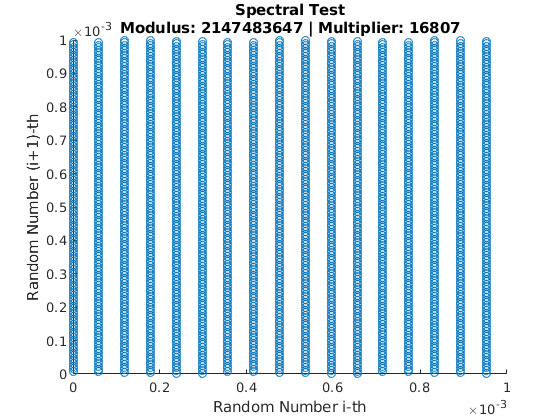
\includegraphics[width=\columnwidth]{fig/evaluation-randomness-spectral-16807}
	\caption{The Spectral Test to evaluate the randomness of the random number generator $(16807,2^{31}-1, 1)$ in the interval $(0, 10^{-3})$.}
	\label{fig:evaluation-randomness-spectral-16807}
\end{figure}

\begin{figure}
	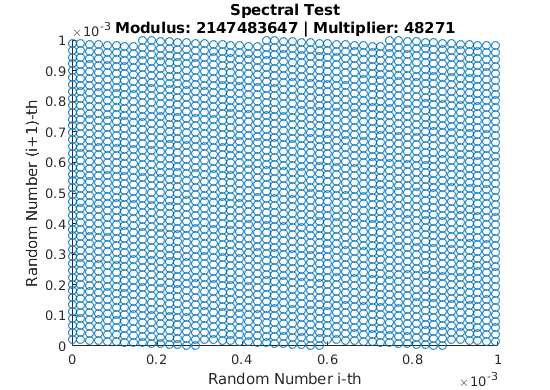
\includegraphics[width=\columnwidth]{fig/evaluation-randomness-spectral-48271}
	\caption{The Spectral Test to evaluate the randomness of the random number generator $(48271,2^{31}-1, 1)$ in the interval $(0, 10^{-3})$.}
	\label{fig:evaluation-randomness-spectral-48271}
\end{figure}

\begin{figure}
	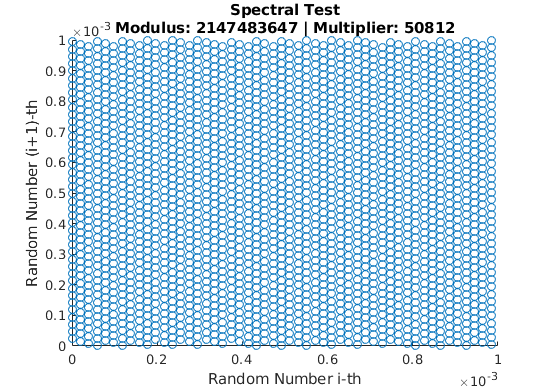
\includegraphics[width=\columnwidth]{fig/evaluation-randomness-spectral-50812}
	\caption{The Spectral Test to evaluate the randomness of the random number generator $(50812,2^{31}-1, 1)$ in the interval $(0, 10^{-3})$.}
	\label{fig:evaluation-randomness-spectral-50812}
\end{figure}

\begin{figure}
	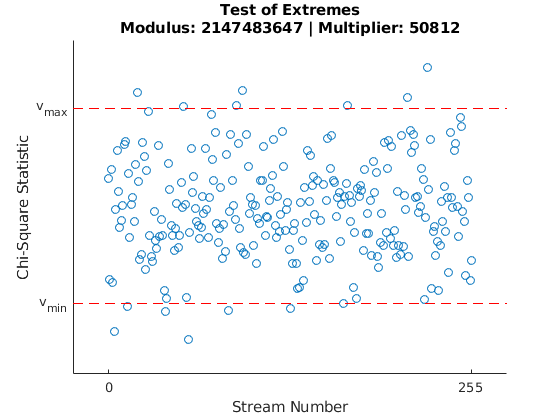
\includegraphics[width=\columnwidth]{fig/evaluation-randomness-extremes-50812}
	\caption{The Test of Extremes with $d=5$ to evaluate the randomness of the random number generator $(50812,2^{31}-1, 256)$.}
	\label{fig:evaluation-randomness-extremes-50812}
\end{figure}

\begin{figure}
	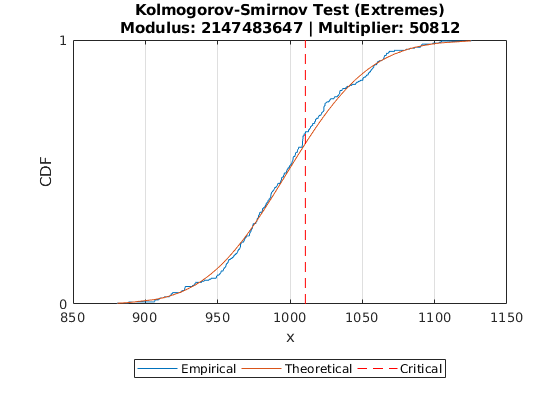
\includegraphics[width=\columnwidth]{fig/evaluation-randomness-kolmogorov-smirnov-50812}
	\caption{The Kolmogorov-Smirnov Analysis (leveraging the Test of Extremes with $d=5$) to evaluate the randomness of the random number generator $(50812,2^{31}-1, 256)$ with $0.95$ confidence level.}
	\label{fig:evaluation-randomness-kolmogorov-smirnov-50812}
\end{figure}


% %
% PERFORMANCE ANALYSIS
% %
\subsection{Performance Analysis}
Let us now consider the experimental results about system performance recorded by our simulator.
In all experiments we considered values stated in Section~\ref{sec:performance-modeling} with a preemption policy based on \textit{random selection}.

\subsection{Transient Analysis}
\label{sec:evaluation-transient-analysis}
First, we conduct a \textit{transient analysis} to evaluate the system stationary in order to (i) prove its convergence to the steady-state and (ii) estimate the duration of the transient period.
%
In fact, given a system that converges to stationary, the knowledge of the duration of the transient period is really important to conduct an effective performance evaluation. In particular, it allows the analyst to focus performance evaluation on a system in its stationary conditions.
%
In the transient analysis we focus on the global system throughput as it can be considered a good representation of the dependency of the system from the initial state.

The following results have been produced by considering an ensemble of $5$ replications, where the $i+1$-th replication is initialized with the last seed of the $i$-th replication, so as to achieve the best decoupling between random sequences of different replications.

In Figure \ref{fig:evaluation-transient-analysis-throughput} we show the transient analysis of the global throughput in the whole system.

The results show that the system reaches the steady-state.
This result is not surprising, because the presence of a stabilizing \textit{infinite-buffer centre}, i.e. the Cloud, largely compensates the possible instability of the \textit{thresholded finite-buffer centre}, i.e. the Cloudlet.

\begin{figure}
	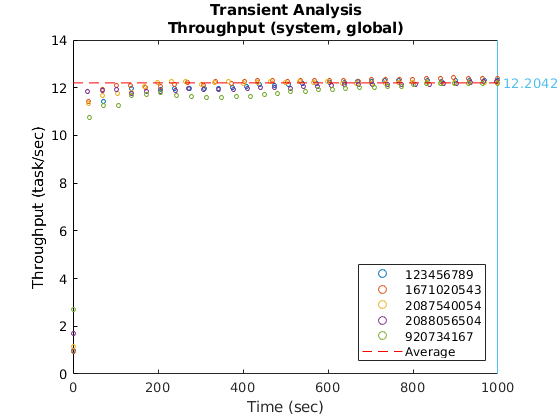
\includegraphics[width=\columnwidth]{fig/evaluation-transient-analysis-throughput}
	\caption{Transient analysis for global throughput in the whole system.}
	\label{fig:evaluation-transient-analysis-throughput}
\end{figure}


\subsection{Performance Evaluation}
Let us now focus on the \textit{performance evaluation}, taking into account the following metrics:

\begin{enumerate}
	\item \textit{response time} both global and classed, both for the system as a whole and for each subsystem;
	
	\item \textit{throughput} both global and classed, both for the system as a whole and for each subsystem;
	
	\item \textit{population} both global and classed, both for the system as a whole and for each subsystem;
	
	\item \textit{interrupted ratio} for tasks belonging to the $2^{nd}$ class.
	
	\item \textit{interrupted response time} for tasks belonging to the $2^{nd}$ class.
\end{enumerate}

In our experiment we assume $S=N=20$, $k=64$ batches, batch dimension $b=512$ and initial seed $iseed=123456789$.
%
Theoretical results have been computed using the formulas presented in Section~\ref{sec:performance-modeling}, assuming the experimentally computed value $E[T_{clt,2,lost}]=1.47445;s.$.

In Table

\begin{figure}
	\begin{center}
		\begin{tabular}{|c||c|c|}
			\hline
			Measure & Theoretical & Experimental\\
			\hline
			$a_{clt,1}$  & $0.978326334857105$ & $0.97911346521$ \\
			$a_{clt_2}$  & $0.603529764734761$ & $0.60502880468$ \\
			$r$          & $0.183573830264005$ & $0.15525744148$ \\	
			\hline
		\end{tabular}
	\end{center}
	\caption{Routing probabilities: comparison between the theoretical result, computed with the analytical model, and the experimental result, computed leveraging our simulator.}
	\label{tbl:evaluation-routing-probabilities}
\end{figure}

\begin{figure}
	\begin{center}
		\begin{tabular}{|c||c|c|}
			\hline
			Measure & Theoretical & Experimental\\
			\hline
			$E[N_{clt}]$  & $123456789$ & $123456789\pm 0.00342$ \\
			$E[N_{clt,1}]$  & $123456789$ & $123456789\pm 0.00342$ \\
			$E[N_{clt,2}]$  & $123456789$ & $123456789\pm 0.00342$ \\
			$E[T_{clt}]$  & $123456789$ & $123456789\pm 0.00342$ \\
			$E[T_{clt,1}]$  & $123456789$ & $123456789\pm 0.00342$ \\
			$E[T_{clt,2}]$  & $123456789$ & $123456789\pm 0.00342$ \\
			$X_{clt}$  & $123456789$ & $123456789\pm 0.00342$ \\
			$X_{clt,1}$  & $123456789$ & $123456789\pm 0.00342$ \\
			$X_{clt,2}$  & $123456789$ & $123456789\pm 0.00342$ \\
			\hline
			$E[N_{cld}]$  & $123456789$ & $123456789\pm 0.00342$ \\
			$E[N_{cld,1}]$  & $123456789$ & $123456789\pm 0.00342$ \\
			$E[N_{cld,2}]$  & $123456789$ & $123456789\pm 0.00342$ \\
			$E[T_{cld}]$  & $123456789$ & $123456789\pm 0.00342$ \\
			$E[T_{cld,1}]$  & $123456789$ & $123456789\pm 0.00342$ \\
			$E[T_{cld,2}]$  & $123456789$ & $123456789\pm 0.00342$ \\
			$X_{cld}$  & $123456789$ & $123456789\pm 0.00342$ \\
			$X_{cld,1}$  & $123456789$ & $123456789\pm 0.00342$ \\
			$X_{cld,2}$  & $123456789$ & $123456789\pm 0.00342$ \\
			\hline
			$E[N_{sys}]$  & $123456789$ & $123456789\pm 0.00342$ \\
			$E[N_{sys,1}]$  & $123456789$ & $123456789\pm 0.00342$ \\
			$E[N_{sys,2}]$  & $123456789$ & $123456789\pm 0.00342$ \\
			$E[T_{sys}]$  & $123456789$ & $123456789\pm 0.00342$ \\
			$E[T_{sys,1}]$  & $123456789$ & $123456789\pm 0.00342$ \\
			$E[T_{sys,2}]$  & $123456789$ & $123456789\pm 0.00342$ \\
			$X_{sys}$  & $123456789$ & $123456789\pm 0.00342$ \\
			$X_{sys,1}$  & $123456789$ & $123456789\pm 0.00342$ \\
			$X_{sys,2}$  & $123456789$ & $123456789\pm 0.00342$ \\
			\hline
			$E[T_{restarted}]$  & $123456789$ & $123456789\pm 0.00342$ \\
			$RestartRatio$  & $123456789$ & $123456789\pm 0.00342$ \\			
			\hline
		\end{tabular}
	\end{center}
	\caption{Performance metrics: comparison between the theoretical result, computed with the analytical model, and the experimental result with level of confidence $95\%$, computed leveraging our simulator.}
	\label{tbl:evaluation-performance-metrics}
\end{figure}

%%
% DISTRIBUTION ANALYSIS
%%
\subsection{Distribution Analysis}
\label{sec:evaluation-distribution-analysis}
In this Section we show the distribution analysis of the Cloudlet global throughput. 
In particular, we focus on both (i) the Probability Density Function (PDF) estimation leveraging distribution fitting, and (ii) the comparison between theoretical and experimental Cumulative Distribution Function (CDF).

In Figure~\ref{fig:evaluation-distribution-analysis-pdf-throughput-cloudlet-global} and  Figure~\ref{fig:evaluation-distribution-analysis-cdf-throughput-cloudlet-global} we show the PDF estimation and the CDF analysis, respectively, for the global Cloudlet throughput when $S=N=20$, where we adopted the \textit{Freedman-Diaconis Rule} for the binning schema.
Results show that the best fitting is the \textit{Normal Distribution} with parameters $\mu\approx7.403$ and $\sigma\approx0.364$.
%
The Normal behavior shown here can be considered as a further good proof of both the system stationary and the effectiveness of the batch means as a tool to study steady-state statistics.

\begin{figure}
	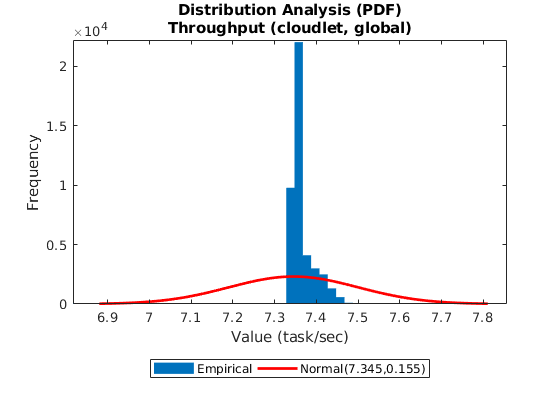
\includegraphics[width=\columnwidth]{fig/evaluation-distribution-analysis-pdf-throughput-cloudlet-global}
	\caption{Distribution analysis (Probability Distribution Function)for the Cloudlet global throughput with threshold $S=N=20$.}
	\label{fig:evaluation-distribution-analysis-pdf-throughput-cloudlet-global}
\end{figure}

\begin{figure}
	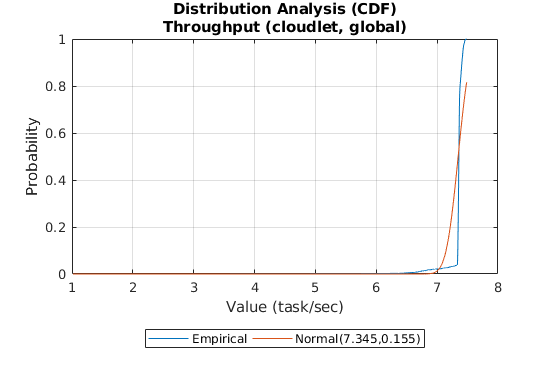
\includegraphics[width=\columnwidth]{fig/evaluation-distribution-analysis-cdf-throughput-cloudlet-global}
	\caption{Distribution analysis (Cumulative Distribution Function) for the Cloudlet global throughput with threshold $S=N=20$.}
	\label{fig:evaluation-distribution-analysis-cdf-throughput-cloudlet-global}
\end{figure}
\section{Conclusions}
\label{sec:conclusions}

\lipsum[1-3]

\appendix
\section{Usage}
\label{sec:usage}


In this Section we show how to configure and run experiments and some sample outputs to provide a better idea of what has been created.

The test of extremes for a custom random number generator produces the output shown in Figure~\ref{fig:usage-randomness-extremes} and can be executed with default configuration by running the script

\begin{lstlisting}
exp/random/randomness/extremes/main.py
\end{lstlisting}

\begin{figure}
	\centering
	\lstinputlisting{ext/randomness-extremes.txt}
	\caption{A sample output of the Test of Extremes.}
	\label{fig:usage-randomness-extremes}
\end{figure}

The test of Kolmogorov-Smirnov for a custom random number generator produces the output shown in Figure~\ref{fig:usage-randomness-kolmogorov-smirnov} and can be executed with default configuration by running the script

\begin{lstlisting}
exp/random/randomness/kolmogorov-smirnov/main.py
\end{lstlisting}

\begin{figure}
	\centering
	\lstinputlisting{ext/randomness-kolmogorov-smirnov.txt}
	\caption{A sample output of the Test of Kolmogorov-Smirnov.}
	\label{fig:usage-randomness-kolmogorov-smirnov}
\end{figure}

The simulation is configured providing a configuration YAML file as the one shown in Figure~\ref{fig:usage-simulation-configuration} and can be executed by running the script

\begin{lstlisting}
exp/simulation/performance/main.py
\end{lstlisting}

\begin{figure}
	\centering
	\lstinputlisting{ext/simulation-configuration.yaml}
	\caption{A sample configuration for a simulation experiment.}
	\label{fig:usage-simulation-configuration}
\end{figure}



%        plain   normal style - listed in ABC order and labeled numerically
%        unsrt   same as plain except entries appear in order of citation
%        alpha   same as plain except entry labels are used
%        abbrv   same as plain except uses abbreviations for first names,
%                month names, and journal names
\begin{singlespace}
\bibliographystyle{apalike}
\bibliography{bib/main}
\end{singlespace}

\chapter{Notes}
\label{chp:notes}

\section{A review of auto-scaling techniques for elastic applications in cloud environments}
\label{sec:lorido2014review}

Notes taken from \cite{lorido2014review}.

Cloud computing environments allow customers to dynamically scale their applications.


\section{Borg, omega, and kubernetes}
\label{sec:burns2016borg}

Notes taken from \cite{burns2016borg}.


\section{Reinforcement learning: An introduction}
\label{sec:sutton1998reinforcement}

Notes taken from \cite{sutton1998reinforcement}.

\end{document}
